%
% Body text font is Palatino!
%

\documentclass[a5paper,pagesize,10pt,bibtotoc,pointlessnumbers,
normalheadings,DIV=9,twoside=false]{scrbook}

% twoside, openright
\KOMAoptions{DIV=last}

\usepackage{trajan}
\usepackage{graphicx}
\usepackage[french]{babel}
\usepackage[utf8]{inputenc}
\usepackage[T1]{fontenc}

\usepackage[babel,french=guillemets]{csquotes}
% \usepackage{librecaslon}
% \usepackage[T1]{fontenc}

\usepackage[sc]{mathpazo}
\linespread{1.05} 

\usepackage{verbatim} % for comments
\usepackage{listings} % for comments

%\setlength{\parindent}{10pt}
%\setlength{\parskip}{1.4ex plus 0.35ex minus 0.3ex}
%\setlength{\parskip}{1.4ex plus 0.35ex minus 0.3ex}

\usepackage{blindtext}
\newcommand{\q}[1]{>>\textit{#1}<<}

\title{A book title}   
\author{Author Name} 
\date{\today} 

\begin{document}
	
	
	%=========================================
	\begin{titlepage}
		\centering{
			{\fontsize{40}{48}\selectfont 
				Comment j’ai évité 52 mois de captivité}
		}\\
		
		\vspace{10mm}
		\centering{\Large{André Trocmé}}\\
		
		\vspace{\fill}
		\centering \large{1991}
	\end{titlepage}
	
	
	%=========================================
	\newpage{}
	\thispagestyle {empty}
	
	\vspace*{2cm}
	
	\begin{center}
		\Large{\parbox{10cm}{
				\begin{raggedright}
					{\Large 
						\textit{A mes enfants et petits enfants}
					}
					
					% 		\vspace{.5cm}\hfill{---Brian W. Kernighan}
				\end{raggedright}
			}
		}
	\end{center}
	
	\newpage
	
	
	%=========================================
	
	Vous m’avez souvent demandé d’écrire le récit de ma vie lors de la guerre 39-45. 
	C’est en octobre 1991 que je me décide à le faire. 
	
	\medskip
	
	Cela commence le 27 août 1939, j’avais 29 ans, j’ai été rappelé à l’armée par un ordre de mobilisation partielle.
	Je suis affecté à la compagnie motocycliste du 67ème Régiment d’Infanterie à Soissons. Là je deviens sous-officier adjoint au lieutenant Debout (qui sera tué devant Stonne en mai 40) commandant d’une section de fusiliers voltigeurs sur side-cars (j’ai un side avec un conducteur).
	
	\begin{figure}[]
		\centering
		\includegraphics[scale=0.4]{./imgs/carte2.pdf}
		\caption{Carte du Nord Est}
		\label{histo_Mt}
	\end{figure}

	\begin{figure}[]
	\centering
	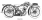
\includegraphics[scale=2]{./imgs/Terrot250.pdf}
	\caption{Terrot 250\,$cm^3$ de type F}
	\label{histo_Mt}
\end{figure}
	
	Dès la déclaration de guerre du 3 septembre nous embarquons pour le S.O. de Rocroi par le train. Nous y restons jusqu’au 10 sept. Avant de gagner la région S.E de Bar-le Duc p.2) (pour moi à Reffroy puis Marsou ?)
	Je suis bien dans la fonction que je remplis.
	Hélas fin octobre les 3 Compagnies Moto des 3 régiments d’Infanterie de la 2ème D.I.M. sont réduites chacune à une section. Je n’en fais pas partie. Presque tout le monde est reparti dans les diverses compagnies. Cette répartition se fait au bureau du colonel. Là j’ai eu ma première chance de cette guerre. Un sergent motocycliste agent de liaison auprès du colonel venait d’être rappelé au Chemin de fer comme « affecté spécial ». Il fallait le remplacer et mon commandant de Compagnie le lieutenant Touhc avec p.3) qui j’étais en bons termes m’a proposé pour cette fonction. Me voici agent de liaison moto sur une Terrot 250 cm3. Je suis chef d’un groupe de 6 motards, des chauffeurs de quelques véhicules tout terrain et des secrétaires du colonel.
	
	Je garderai ma moto jusqu’au 15 juin 40 où sa roue avant sera percée par une balle de mitraillette allemande.
	
	Pour suivre l’action jusqu’à ce jour de juin je vous invite à lire « La 3ème DIM. » par le Général Bertin Boussu. Vous y comprendrez ce que j’ai subi pendant un mois et la chance que j’ai eu de rester vivant. Je ne vous donnerai pas le détail de tout ce que j’ai enduré comme bombardements d’avions et tirs d’artillerie. Je ne vous dirai pas les trouilles que j’ai ressenties parfois pendant des heures, ou toute une nuit à attendre l’obus unique suivant qui tomberait dans 5 minutes (c’est ce qu’on appelle tir de harcèlement)
	
	Je vous rappellerai seulement que le 15 mai 40 j’avais 30 ans et que plaqué au sol qui tremblait sous une pluie de bombes je me disais que ma vie s’arrêterait à 30 ans.
	
	C’est donc sur la route allant d’Arcis-sur-Aube à ………….. , que je me trouvais un peu avant 4h. Le colonel m’avait chargé de poster un pli au P.C.  32 ème ( ?) RI que je devais chercher à l’état major d’Arcis.
	
	Je ne voyais personne sur la route ni aux alentours et je n’entendais que le ronronnement du moteur de la moto quand il m’a semblé entendre des vols d’abeilles  zzzz… J’ai immédiatement compris le bruit des balles. La réaction fut immédiate : couper les gaz, freiner et me jeter sur la route vers le fossé où je fus en un instant.  (P 6) Je me traine sous les arbres qui bordent la route et j’observe au-delà du pré.
	
	Quatre soldats allemands à 100 m s’approchent, nu-tête manches de chemises retroussées, une mitraillette sous le bras. Je suis tendu et je pense à ce qui peut m’arriver. Je crois qu’il vaut mieux ne pas bouger. En restant un peu protégé par un arbre pas plus gros qu’un poteau de téléphone, je lève mon mouchoir au bout de ma main.
	
	Dès qu’ils sont arrivés sur la route ils m’ont vu et se dirigent tranquillement vers moi. J’ai le cœur qui bat mais ils ne me paraissent ni excités ni agressifs (p 7) et les voici près de moi l’arme abaissée. J’en ressens un immense soulagement, j’ai abaissé la main et me suis avancé. Papiers ! dit l’un. Je comprends que voyant un motocycliste ils pensent que je porte un pli (bien sûr le pli que j’avais je l’ai enterré en arrivant dans le bois) aussi je fais l’idiot et je dis ! Ja…en sortant mon livret militaire et mon portefeuille que j’ouvre sur la photo de femme et fille.
	
	-Frau ? 
	
	-Ja ! 
	
	-Krieg, malheur dit le soldat.
	
	Puis nous allons vers la moto. Le pneu avant est à plat, il a été touché par une balle. Les balles ne sont pas (p. 8) passées bien loin de moi et j’ai eu une belle chance d’avoir passé au travers !
	
	On me demande de réparer le pneu. Je ne peux que montrer qu’il n’y a rien sur la moto pour faire le travail. A ce moment arrive sur la route, qui coupe la première, un groupe d’une quinzaine de blessés, allemands et français. On m’envoie à eux et j’aide à soutenir un français blessé à une jambe qu’il faut traîner à deux. 
	
	Nous arrivons bientôt au pont de Vinets que les français ont fait sauter mais imparfaitement et nous le traversons sur les poutrelles démolies. Sur la place du (p.9) village, il y a des troupes et aussi un groupe sanitaire. Un médecin-major nous fait rentrer les blessés dans une maison, où on les couche sur des matelas étendus au sol. Le médecin, voyant mes galons de sergent, me dit en français approximatif de réunir des hommes pour rechercher des matelas dans les maisons. Ce que je fais. Au retour, je suis assailli par un officier à cheval qui doit prononcer des injures et lève sa cravache vers moi. Heureusement, le médecin allemand semble le calmer et il s’éloigne. C’est le seul incident de ma première soirée de prisonnier. Bientôt, nous sommes enfermés dans l’église (p.10) du village déjà pleine de prisonniers. Je pourrai quand même sortir dans la soirée pour visiter des maisons à la recherche de nourriture. Je ne trouverai qu’une bouteille de vin blanc qui me remettra de mes émotions. Je dormirai la nuit, étendu dans la sacristie.
	
	Le 16 mai, départ du convoi à pied. Après 5 heures de marches, nous arriverons au camp militaire de  Mailly. Au cours de la marche, à l’occasion d’un arrêt sur le bord de la route, je recevai un kg de sucre en morceaux du conducteur (p.11) d’un chariot allemand de ravitaillement. Sucre que je partagerai avec mon nouvel ami Pierre Peyramaure avec qui j’ai fait connaissance dans l’église. Il sera presque toujours avec moi et nous reparlerons de lui lors de mon évasion.
	
	Des milliers de prisonniers se rassembleront dans les nombreux casernements du camp de Mailly. J’y suis resté 60 jours, c’est vite dit sur le papier mais ce sont des jours qui ont été bien longs, surtout quand on a le ventre creux. Presque rien à boire et à manger pendant une semaine puis l’organisation s’est faite et le menu a été à peu de (p.12) chose près celui-ci : un jus de je ne sais quoi le matin, une soupe à midi avec quelques haricots rouges des pois et quelques morceaux d’abats de bestiaux (vaches ou chevaux) : poumons, rates- le soir un pain blanc français pour 8 et un bout de fromage (beaucoup de français furent atteints de dysenterie).
	
	Il faisait beau, on se promenait dans le camp en colportant des nouvelles – la libération des prisonniers allait être proche ! –
	
	La nuit on dormait sur les bas-flancs d’une chambre recouverts de paille.
	
	Après le début du mois d’août, des groupes d’une cinquantaine étaient rassemblés et partaient (p.13) on ne sait où (pour être libérés bien sûr !) 
	
	Mon tour vint le 15 août.
	
	Nous nous sommes entassés dans des wagons à bestiaux. Nous avions touché un morceau de pain chacun. Moi j’avais eu une grosse tourte car le distributeur de pain était mon ami le sergent Leurisse, boucher à St Quentin et motocycliste comme moi au 67ème RI- que j’avais la surprise de retrouver là.
	Nous avons roulé toute la nuit avec de nombreux arrêts où nous pouvions entrouvrir la porte pour respirer (p.14) un autre air que celui du wagon où chacun avait pissé ou épanché sa diarrhée dans des boites.
	A l’un de ces arrêts, j’eus la surprise d’être à Tergnier, la gare de mon pays ! Quessy. C’est le cœur bien gros que je repartis, enfermé de nouveau.
	Le matin, long arrêt à Amiens puis fin du parcours à Doullens.
	Là nous sommes parqués dans un pré entouré de barbelés, pendant une semaine au régime des débuts de la captivité c.à.d. presque rien. (p.15)
	Enfin départ en camions et arrivée d’une centaine de prisonniers dans une grande ferme à St Lô. Bientôt arrivent les maires des communes voisines avec leurs secrétaires de mairie. Il leur faut à chacun 20 à trente prisonniers pour fournir leur village en aides agricoles/ je fais la connaissance de l‘instituteur de Maison-Ponthieu et je deviens chef de Kommando de cette commune. Chaque matin, j’emmènerai mon groupe de 25 hommes au village et le ramènerai pour la nuit à la ferme de St Lô où nous couchons à terre dans les écuries. Ceci pendant une quinzaine. Puis ordre de rester à demeure chez les habitants. Je pus écrire à Quessy et à St Dizier et recevoir pour la 1ère fois des nouvelles des miens. 
	(p.16) Le matin les prisonniers se rassemblaient sur la place du village, je faisais l’appel et allait en rendre compte au commandant allemand du camp de St Lô (un caporal avocat dans le civil qui parlait bien le Français). Je restai à Maison-Ponthieu jusque vers le 5 octobre. Bien nourri chez l’instit. J’avais repris du poids et meilleure mine ainsi que bon moral. Même votre mamie était venue me voir.
	C’est là que j’eus (p. 17) une idée saugrenue. J’achetai pour 50 f un brassard de la Croix-Rouge, falsifiai mon livret militaire et fis une demande de libération traduite en allemand que je remis au chef de St Lô pour qu’il l’envoie au chef du Stalag 172 à Abbeville dont nous dépendions. La réponse ne se fit pas attendre : j’étais muté au Kommando de Neuville-Oneux à une quinzaine de km de là. Quelle déception ! Pendant mon séjour à Maison-Ponthieu, seuls 2 prisonniers ne s’étaient pas présentés à l’appel du matin. J’en avais rendu compte et on ne s’en était pas trop affecté. (p.18) Je pensais depuis un moment à en faire autant. Dès mon arrivée à Neuville cette idée s’intensifia.
	Je réussis à m’incorporer à un groupe qui allait travailler à Domqueur. Mais on rentrait encore chaque soir au camp. J’oubliais de vous dire qu’en arrivant à Neuville je déclinai mon identité au bureau français. A l’interrogation : votre domicile ? je répondis (dans la marge Zone non occupée*) St Dizier-Leyrenne (Creuse) au lieu de Quessy-Cite (Aisne) avec la petite idée que si je m’évadais on ne me recherche pas dans l’Aisne zone occupée. Aussitôt un prisonnier, assis près du bureau, (p. 19) se lève et s’étonne : tu es de St Dizier, moi du Compeix. Nous faisons connaissance : C’est George Blanchon. Je vous en reparlerai bientôt.
	Revenons à Domqueur. Au bistrot où nous atterrissions chaque matin je m’étais renseigné sur une possibilité d’accueil dans une famille et le mastroquet m’avait désigné un bonhomme assez seul à une table dégustant son rhum. C’était Monsieur Leroy, un veuf assez agée.
	Je l’abordai et lui proposai de venir chez lui chaque jour où je lui donnerais 5 F pour le repas de midi. Je fus assez convainquant pour qu’il accepte. Et quelques jours plus tard quand nous fûmes autorisés à coucher chez l’habitant, il m’offrit (p.20) un lit dans une petite chambre. Quand sa fille (Oni) dix ans rentrait de l’école je m’occupais de ses devoirs et de ses leçons, travail fort apprécié par ses tantes qui habitaient un peu plus loin et me gâtait beaucoup. C’était mon seul travail de la journée. Les repas étaient préparés par la jeune bonne de M. Leroy, Sophie, une polonaise. Elle me prêtait son vélo et j’allais même avec mon brassard Croix-Rouge jusqu’à Abbeville pour me faire photographier (carte d’identité) sans jamais être interpellé. 
	(p. 21) Dès mon installation à Domqueur j’avais écrit à Mamie pour qu’elle m’envoie linge et vêtements civils par colis séparés tous les 2 jours. Je n’étais pas pressé mais c’était décidé j’allais m’évader. J’avais caché un « Chaix » et établi mon itinéraire : il ne fallait pas franchir la Somme vers le sud car c’était la frontière de la zone interdite très surveillée par les Allemands. Je prendrais le train à Conteville à 6 km de Domqueur me dirigeant vers Douai puis sur St Quentin en zone interdite aussi. J’ouvre une parenthèse pour vous dire qu’à Maison -Ponthieu j’avais eu des nouvelles d’un copain évadé qui avait rejoint une amie en Saône et Loire. Il me donnait son adresse : Les Brosses Chassenard par Digoin et m’incitait à la rejoindre pour me faire passer en zone libre, juste à sa porte.
	Les jours passaient, les colis arrivaient. Il ne manquait plus que les chaussures quand un matin à l’appel, (p. 22) il était fait chaque jour par les Allemands, on nous interdit de repartir. C’était la catastrophe. Les paysans furent prévenus par le garde-champêtre, ils nous apportèrent nos affaires personnelles. Puis nous regagnons Neuville-Oneux où se rassemblèrent tous les hommes des communes environnantes. Nous y restons 3 jours.
	La brave Sophie m’y apporta deux fois une baguette de pain. Tout ceci se passait au début décembre 1940. Dois-je vous dire que je me rongeais les sangs : Louper une évasion pour un retard de 2 jours. Mais j’avais (p.23) beau tourner en rond je ne voyais aucune issue.
	Le départ pour Abbeville arriva : 12 km à pied, bien encadrés par les sentinelles.
	Là, je fais connaissance avec un vrai camp de prisonnier le frontstalag 172A (Doullens). C’est parait-il un ancien camp des troupes anglaises du début de la guerre : 20 à 30 baraquements en bois que les Allemands ont entourés d’un double mur de grillage à 3 ou 4 m l’un de l’autre, de 3 m de haut et remplis à l’intérieur de gros boudins de barbelés. A l’extérieur des tours en bois : les miradors. 
	(p. 24) C’est là que pendant 8 jours (je ne me souviens plus exactement du temps et des dates tellement j’étais oppressé de me trouver là, n’ayant pas eu l’intelligence de partir plus tôt. Je tournais en rond me torturais l’esprit pour trouver une solution refusant cet enfermement, échafaudant des plans irréalisables et ne (p. 25) trouvant rien pour en sortir. Il ne restait plus qu’à attendre le départ pour l’Allemagne. J’ai oublié de vous dire qu’en arrivant au stalag avec mon brassard un adjudant français s’était approché de moi pour me dire de prendre contact avec lui pour une libération possible des « sanitaires »-ce qui fut fait.
	Justement, un jour, cet adjudant me dit : « Chaque matin une corvée de quelques hommes va vider les tinettes des chiottes allemandes, voulez-vous la commander demain matin ? » J’accepte donc et le 13 décembre vers 9h nous passons devant la sentinelle allemande qui lève la barre comme celle d’un passage à niveau. Nous sommes dans la cour de la garde de camp : un bâtiment en face, un à gauche et un à droite se touchant en u. Vers la gauche il (p.26) y a un chemin, au-delà des barbelés du camp, qui va vers la ville. A droite, fermé par une porte à barreaux, un étroit chemin. Une sentinelle armée vient au-devant de nous et nous ouvre cette porte. Nous suivons le chemin qui longe l’extérieur de la baraque et arrivons derrière celle du fond. : le casernement allemand. Il n’y a aucune porte ni aucune fenêtre, simplement au niveau du sol peut-être 6 trappes qui se soulèvent. La sentinelle ne nous a pas accompagnés. Je m’en étonne : « Quelques fois ils viennent, quelquefois pas » Les prisonniers ouvrent les trappes et je vois sous chacune un cuvier en bois qui se remplit à mesure des besoins des soldats. Toute cette « merde » est vidée dans un fossé et on la recouvre de terre. Pendant ce travail mon esprit a beaucoup travaillé. Personne ne nous voit. Il y a un angle mort important pour la sentinelle du prochain mirador. Si on a assez de sang froid pour s’éloigner lentement, on ne doit pas attirer son attention.
	Voilà ce que je me dis toute la journée du 13. Je suis malgré la témérité de l’entreprise absolument décidé à partir le lendemain. Je persuade Blanchon d’échanger son pantalon en toile bleue contre le mien en drap kaki (qui sera bien plus chaud pour l’hiver !) (p.28) Je vais voir Peyramaure qui était resté à Maison-Ponthieu et que j’ai retrouvé au stalag. Il faut qu’il me trouve un veston civil. A force de parler avec les copains de son baraquement, il m’en trouve un que j’acquière pour 50 francs.
	Faut-il vous dire que j’ai bien mal dormi cette nuit du 13 et 14 mais j’étais tellement anxieux à l’idée de partir en Allemagne que j’acceptais de tout risquer. (p.29) J’essaye de me mettre à la place de l’Allemand du mirador. A part le camp il avait un immense champ autour de lui. Personne ne peut essayer de passer les barbelés, aussi c’est tranquille. Il n’est forcément pas attentif à ce qui se passe dans les champs. Et puis des civils français peuvent y passer. (p.28)
	14 décembre au matin. Jour froid et brumeux. Au plus tôt, je retrouve mes hommes auxquels j’adjoins Blanchon. Même scénario que la veille : une sentinelle nous ouvre la porte et … nous suit derrière les bâtiments : jugez de ma déception. Tout est foutu.
	(p.29) Le travail terminé, elle nous ramène devant. Je la vois fermer la porte à clef, la reporter au bureau, rentrer dans son casernement.
	Je suis remonté à fond, il faut agir et essayer de nouveau. Je demande aux hommes d’aller chercher des seaux de chaux et de revenir. Personne dans la cour des gardiens. La sentinelle soulève sa barre. Nous faisons « Attendez-moi ! » (p.30) J’entre au bureau où je ne suis jamais allé. Le gradé est à son bureau avec un scribouillard. Je dis « Clef pour chaux dans les latrines ». Il me montre une clef sur un grand tableau. Je m’en saisis. Ja ! fait-il. Retour dans la cour. Aucun Allemand. « En avant les gars ! » Serrure ouverte puis refermée derrière nous. J’ai le cœur qui bat à 150. Cette fois je vais me jeter à corps perdu dans l’action. J’ôte mon pantalon (?) kaki que Blanchon enfile. Un béret sur la tête, je suis un civil. « Salut les gars » : Ils ne semblent pas bien comprendre. Blanchon reportera la clef au bureau. 
	(p. 31) Je m’éloigne le plus tranquillement possible de la baraque mais en infléchissant plutôt à droite du mirador. A un moment, je sais que je ne suis plus à l’abri des vues. « S’il y a un coup de feu, touché ou pas je me jette à terre ! » Rien. J’ai un culot terrible : Je m’arrête par moments, me baissant pour ramasser un caillou ou une plante. Progressivement je change ma direction pour partir vers la gauche. Je ne suis pas du tout rassuré mais je progresse prenant peu à peu la direction de la grande route qui est à 2 ou 3 cents mètres. Cette fois je m’en approche vraiment. Mon pas se fait plus sûr. (p.32) La route est bordée de pavillons assez isolée les uns des autres. Cette fois, il me semble que j’ai gagné. Pas un regard en arrière pour voir mes camarades abandonnés. La maison qui est devant moi a une fenêtre ouverte. Elle n’a pas de clôture derrière. Il y a juste à ma gauche un grillage que je suis puis devant moi sur la rue la porte grillagée. Un regard à droite pour voir si quelqu’un intervient ! une fenêtre ouverte mais personne. Il y a une serrure mais elle n’est pas fermée. C’est la porte de la liberté. Quel Ouf ! je lâche, Oui je suis vraiment libre. Il y a quelques piétons sur le trottoir, je me dirige vers la ville ! Il me semble que je n’ai jamais été aussi heureux. Bientôt j’arrive à l’entrée du chemin (p. 33) qui mène au camp. Il y a une sentinelle armée à la porte. Qu’est-ce que je ressens : un immense plaisir, un soulagement d’avoir quitté un monde de prisonniers et aussi une fierté d’avoir réussi un coup aussi risqué. 
	Un carrefour à l’entrée de la ville et un petit bistrot : j’y entre résolument pour m’asseoir à une table et commander « un cognac » J’en avais bien besoin! Des ouvriers français et des Allemands au comptoir. Je peux maintenant réfléchir calmement à ce qu’il me reste à faire. J(ai fait connaissance à Domqueur d’un homme (tchèque je crois) qui travaille  à Abbeville dans une maison de matériel agricole. Je me renseigne et je m’y rends. La dame qui me reçoit me dit qu’il ne vient pas le samedi. Je lui dis (p. 34) mon intention de me rendre à Domqueur. « Tous les samedis dit-elle, le boulanger de Domqueur vient chercher de la farine chez son frère boulanger aussi. Vous allez certainement le trouver ». « La chance est avec moi aujourd’hui » Renseigné sur cette boulangerie, je m’y rends. Une toute jeune fille se présente. J’achète un petit pain et parle du boulanger. Sa maman est appelée et me confirme la venue du beau-frère l’après midi. J’en suis à mon 2ème petit pain. On s’étonne de mon appétit et devant (p. 35) la mine avenante de ces femmes (Il y a une 2ème soeur qui est entrée) je me laisse aller « je viens de m’évader du camp de prisonnier ». C’est le triomphe, on me fait entrer, on appelle le boulanger. Je dois tout raconter ! Et je suis invité à dîner. Comme tout change vite dans la vie ! Hier malheureux, aujourd’hui fêté.
	Vers 4 heures arrive la petite camionnette, chargement des sacs et départ pour Domqueur (Je suis avec les sacs). Un soldat allemand qui fait du stop est embarqué en route. Il descendra peu après. Une fois arrivé, je vais chez la famille Leroy bien étonnée. Monsieur Leroy a bien un peu peur mais je serai tout de même bien accueilli. (p. 36) Après une nuit de repos, me voilà le dimanche 15 décembre en tenue de ville, chaussures fines bien cirées. Adieux aux Leroy. Et 7 km à pied pour prendre mon train à la petite gare de Fonteville. J’ai bientôt un train qui me mène plus au Nord à St Pol-sur-Ternoise (Pas-de-Calais). J’entre dans un restaurant où on me sert une excellente omelette que je mange au milieu de beaucoup de soldats allemands (grosse satisfaction intérieure de pouvoir les côtoyer d’une autre façon qu’au camp !) Il n’y a pas d’hôtel mais on m’indique une femme qui accepte de loger des voyageurs. Après une nuit dans de beaux draps, je prends le train pour Arras et Douai. La circulation des civils dans les gares et les trains s’y fait librement comme avant guerre.
	(p. 37) Pour comprendre mon itinéraire, sachez que les Allemands ont crée une zone interdite comprenant les départements du Nord Pas-de-Calais, Ardennes- Nord de l’Aisne et de la Somme gardée et interdite de passage réglementé. 
	A Douai, je prends un train vers l’Est pour gagner Busigny ou passe l’express Bruxelles-Paris.
	Sur le quai de Busigny : des civils français et aussi des militaires allemands. Je vois au bout du quai, une patrouille de trois Feld-gendarmes. J’ai bien une carte d’identité faite par moi-même seulement pour me rassurer mais je ne tiens pas à ce qu’on me la demande. (p. 38) Voici un officier allemand, je lui demande l’heure bien poliment et j’essaye d’engager la conversation. Ce qui réussit parfaitement. Les feld-gendarmes passeront en saluant et n’auront pas l’idée de demander les papiers à un homme en compagnie d’un officier. Il va à Paris et je le quitte à l’arrivée du train pour monter en 3ème classe. Je descends à St Quentin. Je suis toujours en zone interdite mais je vois un soldat à l’entrée du hall de la gare qui contrôle les pièces d’identité. Il vaut mieux l’éviter. Aussi je longe une rame à l’arrêt vers les bureaux et accoste (p. 39) un employé. Je lui montre mon billet et lui demande de me faire sortir par les bureaux, ce qu’il accepte de faire. St Quentin : c’est là que j’ai passé mon enfance. Après avoir bu mon premier Viandox dont j’avais envie depuis longtemps, je gagne à l’autre bout de la ville la rue Edmond Rostand où habitent mes parents. Je les surprends bien sûr et quelle joie pour eux de me retrouver alors qu’ils me croyaient parti en Allemagne. J’ai deux lettres à faire, une à Mamy pour la rassurer car elle n’a plus de nouvelles depuis mon entrée au Stalag (p. 40) et une autre au copain de Saône et Loire, avec qui je prends rendez-vous à la gare de Digoin pour le mardi 24 au soir afin qu’il me fasse passer la ligne de démarcation. 
	Mamie vient me chercher à St Quentin le dimanche 22 pour rentrer a Quessy-Cité. Elle m’a fait faire une carte d’identité à la mairie de Quessy. En descendant à la gare de Tergnier on n’est plus en zone interdite comme à St Quentin, mais il faut un ausweis pour passer. Mamie en a un mais pas moi. Tant pis, nous passons dans la foule des voyageurs que la sentinelle a du mal à contrôler. Mamie montre son ausweis et dit c’est mon mari en m’entraînant par le bras. Je rentre enfin chez moi 4 rue du Stade.
	(p. 41) Le lendemain matin, lundi 23 je tiens à prendre le 1er train pour Paris avant le jour. Mamie me rejoindra après la classe du soir. La sonnerie du réveil a bien été mise sur 5 h. mais il a oublié de sonner ; nous avions oublié de remonter le mouvement du réveil. Je pris un train dans la matinée et après avoir passé la journée chez Tintin Martineau je retrouverai mamie à la gare du Nord. Une nuit à Paris et départ le 24 pour Moulins en zone occupée où je dois changer de train pour Digoin-toujours en zone occupée. Arrêt à Moulins, nous nous apprêtons à descendre. Mais (p. 42) un haut-parleur annonce qu’il est interdit de descendre du train. Le contrôle se fera dans le wagon. Attente. Des officiers arrivent, demandent les papiers que nous montrons. Je leur déclare que je ne vais pas en zone libre mais que je veux descendre à Moulins. Après visite des bagages on me dit d’attendre dans le wagon : « Vous descendrez quand l’ordre sera donné » Je ne comprends pas cette façon de contrôler mais enfin. C’est longtemps après que le train est enfin contrôlé en entier. Alors le haut-parleur annonce : « le contrôle est terminé ; les voyageurs pour Moulins peuvent descendre » Je m’apprête à le (p. 43) faire, mais le mot « peuvent » me taquine l’esprit « peuvent…mais s’ils ne veulent pas ? » Je dis à mamie ! on reste. Je pense qu’ils ne referont pas un 2ème contrôle au départ. En effet peu après le train s’ébranle. Je demande à un voyageur qui lui, avait un laissez-passer : « Est-ce loin la ligne de démarcation ? »
	- non, nous sommes au-dessus » C’est ainsi que bien bêtement nous avons franchi la Ligne pour la 1ère fois. Les gens du poste-Frontière de Moulins n’étaient pas bien fûtés. Mais ils changeront leur (p. 44) manière de faire car j’eus l’occasion de franchir encore cette ligne, mais il fallait descendre à Moulins pour demander un laissez-passer à la Kommandanture. Après un supplément de parcours payé au contrôleur sans commentaires de sa part j’arrivai à Vieilleville le 25 décembre 40 au soir. Puis après 7 km à pied, enfin St Dizier où la Famille, ma fille Colette en tête nous dit son bonheur, tempéré par l’absence de Pierre toujours en Allemagne. Et dire que ç’aurait dû être mon lot ! J’allais gagner plus de 4 ans de vie- sur un coup de poker-
	Après le 1er janvier, je conduisis mamie jusqu’aux Brosses-Chassenard où la (p. 45) dame qui habitait en bordure du canal était connue des sentinelles, passait journellement en laissant quelques friandises et pouvait avoir une amie avec elle.
	Je regagnai seul St Dizier pour me faire démobiliser à Guéret, voir l’inspecteur d’Académie qui me nomma instituteur à Sardent après un mois de repos.
	Aux grandes vacances votre mamie put venir me rejoindre avec un ausweis obtenu à Moulins (télégramme envoyé de St Dizier « Mère malade » envoi autorisé seulement après certificat du médecin et signature du maire).
	En septembre mamie repart seule par l’itinéraire de Moulins. (p. 46) Moi je décide de rentrer à mon poste de Quessy-Cité. Les conversations avec des personnes qui y sont passées m’apprennent que le poste frontière, sur la route au sud de Bourges est assez conciliant. Je vais m’y diriger par le train. Il y a plusieurs changements de train et au dernier changement j’apprends que le train que j’attendais ne circule pas le dimanche. Je ne veux pas attendre le lendemain et je pars à pied (35 km) J’arrive épuisé et m’affale sur la banquette en bois d’un café. Je trouverai à manger, une chambre mais pas d’encouragement de la part de la population. Beaucoup de candidats au passage ont été refoulés. Tant pis.  Je rejoins (p. 47) la route de Bourges. Au poste de garde isolé au bord de la route en pleine campagne. Je montre ma carte d’identité de Quessy. Je suis allé voir ma femme malade au Sana de Guéret et je voudrais rentrer chez moi où je suis instituteur. « Gut ! passez » Je veux offrir des oeufs que j’ai dans ma petite valise 
	- Merci mais on n’en manque pas. » 
	A chaque vacances, mamie et moi avons réussi à obtenir un laissez-passer à la Kommandantur de Moulins avec notre fameux télégramme : mère malade.
	Mais pour éviter les (p. 48) procédures difficiles d’envoi de St Dizier, je trouvai un truc plus simple. Je me rendais à vélo à la poste de Charmes, à 10 km de Quessy. Un télégramme : Expéditeur : Monthioux à Charmes – Destinataire : Trocmé à Quessy (Aisne) Texte « Mère gravement malade Médecin demande présence des enfants »
	J’avais remarqué que sur le télégramme distribué il n’était pas mentionné le département du lieu d’expédition. Je pouvais donc à Moulins muni de mon télégramme bien authentique demander un laissez-passer pour me rendre à Charmes (Puy-de-Dôme) (p. 49) Nous avions même fait connaissance à la kommandantur d’un lieutenant qui correspondait avec une infirmière de Quessy (Souvenir de leurs études à Paris) Il ne faisait pas de difficultés ayant un télégramme pour le couvrir à accepter notre demande pour un passage valable 2 mois.
	Mon dernier passage vers le Sud se fit à vélo de St Quentin à St Dizier (530 km) du 13 au 17 juillet 1944. Mais là, il n’y avait plus de frontière. Je dus présenter ma carte d’identité à une sentinelle sur le pont de Giens- et à la sortie de Guéret le 17 au soir. Le 18 en m’éveillant à St Dizier, je retrouvai (p. 50) les Allemands autour de la maison. Une division qui remontait vers la Normandie traquait le maquis. Il me fallut m’expliquer avec un sergent qui parlait heureusement bien le français (je pense à un Alsacien) C’était la dernière fois que je voyais les troupes allemandes. 
	A mon retour à St Quentin, le 30 septembre 1944, il restait peu de la France à libérer.
	Pierre avait encore 7 mois à tirer, ainsi que Blanchon et Peyramaure. ! Ils ne rentreront qu’en mai 1945. Il avait 35 ans et moi aussi. Je vous embrasse bien et vous souhaite une vie exempte de guerre.
	Pages 51 et 52  barrées – pages 52 à 67 absentes -
	(p. 67) Colette fut ramenée avec nous à Quessy en septembre 42. Et puis mamie tombe malade. Les soucis, les restrictions alimentaires avaient entamé sa santé. Elle me quitta en emmenant Colette en février 1943. 
	Alors qu’elle se soignait à St Jean d’Aulp, je pus aller la voir à Noël 1943 puis à Pâques 1944 (mais cette fois avec une autorisation spéciale du sous-préfet de St Quentin pour entrer dans cette zone interdite à cause des combats avec les maquis de Haute Savoie) (p. 68 barrée)
	(p. 69) Je ne terminerai pas sans une pensée à mon copain de Maison-Ponthieu qui s’évada le premier et qui en me donnant un point de passage de la ligne de démarcation fut à la base de mon évasion. C’est chez lui aussi – ou plutôt chez une amie que passèrent toutes les lettres sous double enveloppe  entre St Quentin et St Dizier. En effet la circulation du courrier était libre à l’intérieur des zones, elle était interdite d’une zone à l’autre ou plutôt limitée l’envoi de cartes spéciales sous enveloppe avec peu de place pour la correspondance. Nous envoyons nos lettres aux Brosses-Chassenard par Digoin (Saône et Loire) dans la zone occupée ou par Le Pin (Allier) pour la zone libre. Mme Julie Méraud  -dans la marge Louise Meyneau (je ne suis plus sûr du nom)- assurait le passage des lettres dans l’autre zone.
	
	
	Post-scriptum   le 8 . 1 . 92
	A Frédérique, Olivier, François
	Vos parents sont passés.
	Après avoir lu ce mémoire et en retournant en Haute Savoie le 28 . 12 (écrit en chiffres romains) dernier, vos parents ont voulu trouver trace de notre passage au Sud de Digoin en janvier 41. Et ils ont trouvé !  Hélas la dame dont il est question en fin de mes écrits est morte en 90. Mais sa fille les a reçus et ils ont évoqué ensemble cette période d’avant sa naissance dont sa mère lui avait parlé. 
	
	%=========================================
	\begin{comment}
	Just some notes, not visible in pdf.
	\end{comment}
	
	
\end{document}
